\documentclass[../homework.tex]{subfiles}

\pagestyle{fancy}
\fancyhf{}
\rhead{Hanzhi Zhou}
\lhead{Physics 2415 Homework}
\cfoot{\thepage}

\begin{document}
\subsection{Problem 9.1}
\subsubsection*{a)}
\begin{figure}[H]
    \centering
    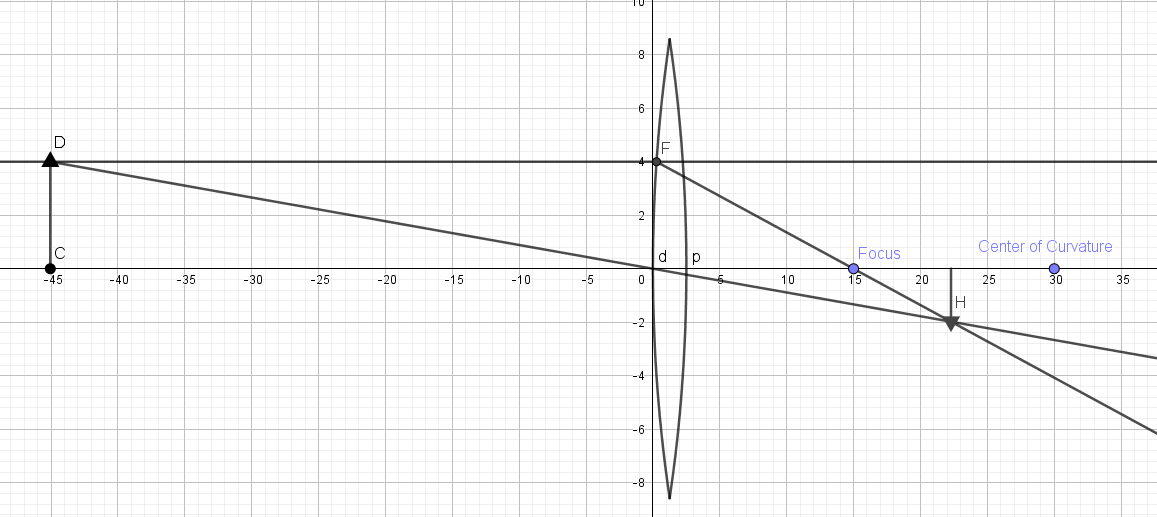
\includegraphics[width=\columnwidth]{p1-a.png}
\end{figure}
\begin{equation*}
    d_i = \left(\frac{1}{15} - \frac{1}{45}\right)^{-1} = \frac{45}{2}
\end{equation*}
\begin{equation*}
    M = -\frac{45/2}{45} = -\frac{1}{2} 
\end{equation*}

\subsubsection*{b)}
\begin{figure}[H]
    \centering
    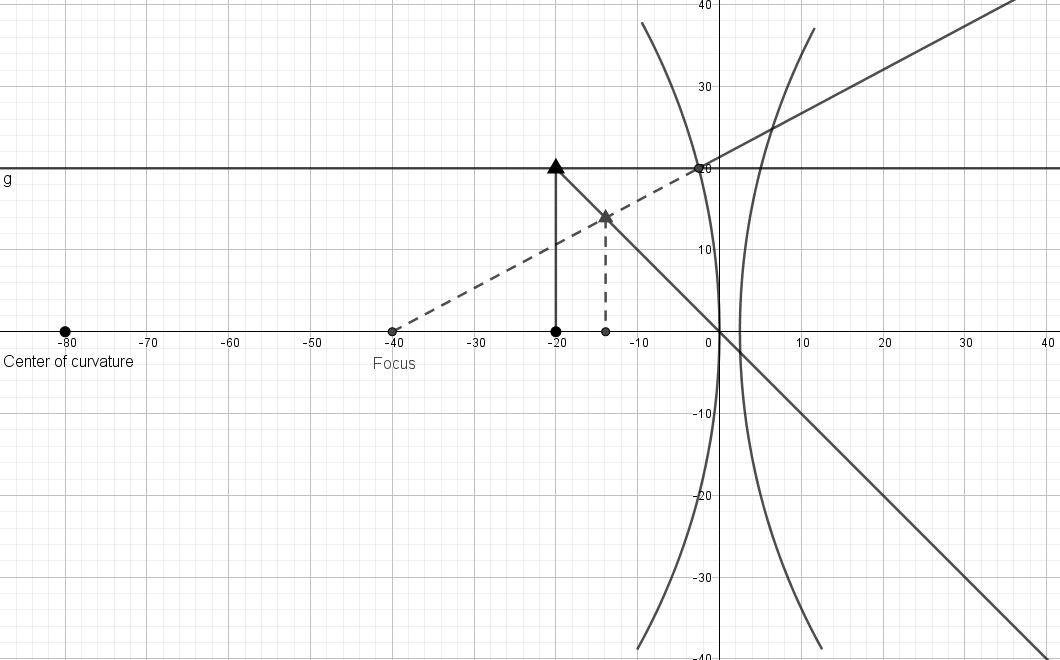
\includegraphics[width=\columnwidth]{p1-b.png}
\end{figure}
\begin{equation*}
    d_i = \left(\frac{1}{-40} - \frac{1}{20}\right)^{-1} = -\frac{40}{3}
\end{equation*}
\begin{equation*}
    M = -\frac{-40/3}{20} = \frac{2}{3} 
\end{equation*}

\subsubsection*{c)}
\begin{figure}[H]
    \centering
    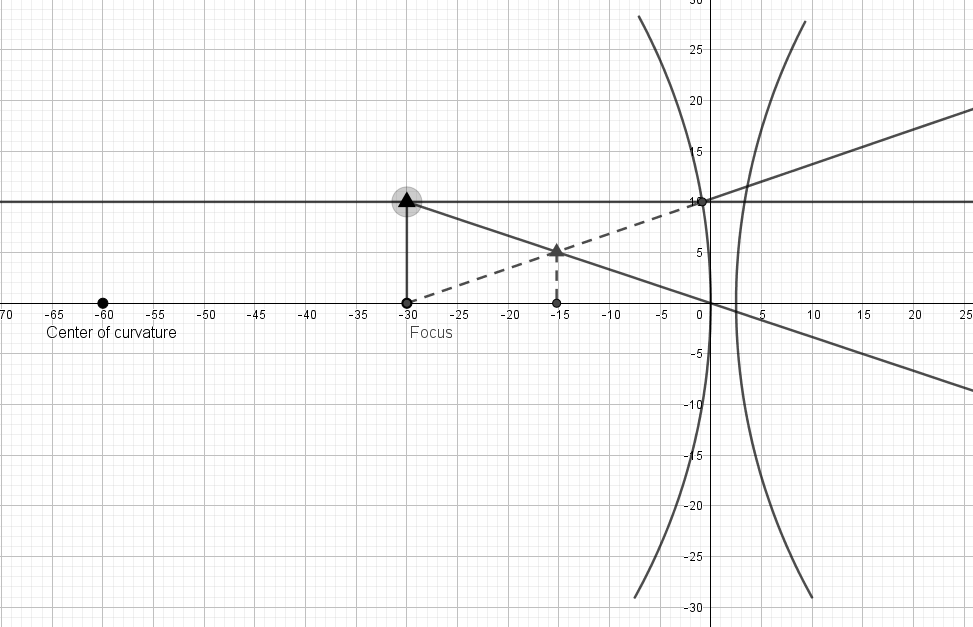
\includegraphics[width=\columnwidth]{p1-c.png}
\end{figure}
\begin{equation*}
    d_i = \left(\frac{1}{-30} - \frac{1}{30}\right)^{-1} = -15
\end{equation*}
\begin{equation*}
    M = -\frac{-15}{30} = \frac{1}{2}
\end{equation*}

\subsubsection*{d)}

\end{document}